\documentclass[xcolor={usenames,dvipsnames}]{beamer}

\mode<presentation> { }

\usetheme{metropolis}
\usepackage{listings}
\usepackage{polyglossia}
\setmainlanguage{english}


\usepackage[numbers]{natbib}

\usepackage{tikz}
\usetikzlibrary{arrows, decorations.pathmorphing,backgrounds,fit,positioning,shapes.symbols,chains, positioning,automata}

\usepackage{lstc}
\usepackage{lstnasm}
\renewcommand{\lstcurrentinputdir}{listings}

%settings 
\everymath{\displaystyle}

\title{Dynamic libraries explained }
\subtitle{as seen by a low-level programmer}
\author{I.Zhirkov}

\date{2017}

%\AtBeginSection[]{
%    \begin{frame}<beamer>{}
%        {\huge \secname}
%    \end{frame}
%}
\AtBeginSection[]
{
  \begin{frame}<beamer>{\secname}
    \tableofcontents[currentsection, currentsubsection,
      subsectionstyle=show/show/hide, sectionstyle=show/show]
  \end{frame}
}


\iffalse
Этот мини-курс посвящен устройству динамических библиотек на низком уровне в современном 64-разрядном окружении. Будут рассмотрены следующие вопросы:

— Зачем нужен компоновщик и динамический загрузчик. 
— Релокация. 
— Структура ELF-файлов: секции, сегменты. Таблицы символов. 
— Отличие статического и динамического связывания. 
— Position Independent Code.
— Global Offset Table и Program Linkage Table. 
— Как описывается интерфейс динамических библиотек. 
— Процесс разрешения символов. 
— Оптимизация динамических библиотек. 
— Small, Medium, Large Code Models и как они изменяются в условиях Position Independent Code. 

\fi

\begin{document}

\begin{frame}
  \titlepage
\end{frame}


\begin{frame}{Exemplary environment}
    \begin{itemize} 
        \item  Intel 64 aka AMD64 aka x86\_64.
        \item  GNU/Linux
        \item  Object file format: ELF files.
        \item Languages: C, Assembly (NASM)
\end{itemize} 
\end{frame}


\section{What is linking?}
\subsection{Compilation}

\begin{frame}{\subsecname}
    \begin{itemize}
 \item  Compiling code is not trivial.
 \item  One of challenges -- carefully placing code and data in memory.
\end{itemize} 
\end{frame}

\begin{frame}[fragile]{Example}

    \begin{tabular}{p{5.3cm} c}
        {
        
\begin{cexample}
int x;
int y;

void f() {
    x = x + 1;
}
\end{cexample}


        \only<2>{
       
\begin{itemize}
    \item  Where to place \c{x} and \c{y}?
    \item  Instructions need to know data addresses. 
    \item  \emph{Once an address is picked, it is difficult to change.}
\end{itemize}

        }

        }&{
            \raisebox{-\height}{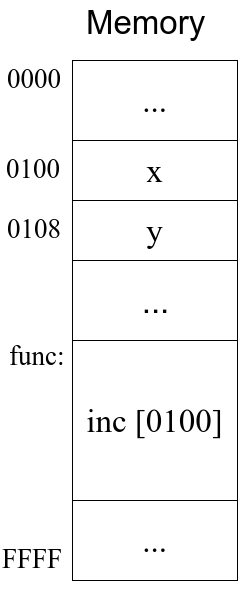
\includegraphics[scale=0.3]{images/relocation-1.png}}
        }
    \end{tabular}

\end{frame}



\begin{frame}{Solution: linking stage}
    \begin{itemize}
 
\item  Defer placement until the last stage of compilation.
    \begin{itemize}
 \item  Instructions generated, we know all functions and global variables.
    \end{itemize} 
\item  Program entities which make sense for linking are called \textbf{symbols}.
\end{itemize} 

\end{frame}



\begin{frame}[fragile]{Symbols}

For each symbol we know its:
    \begin{itemize}

        \item  Name
        \item  Address if assigned
        \item  Where it is referenced.
\end{itemize} 
     Assigning addresses to symbols is called \textbf{relocation}.

\begin{cexample}
int x;          // symbol 'x'

void f() {      // symbol 'f'
    x = x + 1;  // symbol 'x' referenced
}
\end{cexample}


\end{frame}

\begin{frame}{Need for separate compilation}
    \begin{itemize}
        \item Most useful programs are too big for one file (should split into modules.
        \item Need to use code that is already compiled (libraries).
        \item  Don't recompile everything after each change (debug time explodes).
            \begin{itemize}
                \item  Some programs take \emph{hours} to compile.
            \end{itemize}
    \end{itemize} 

\end{frame}


\begin{frame}{Compilation pipeline}
    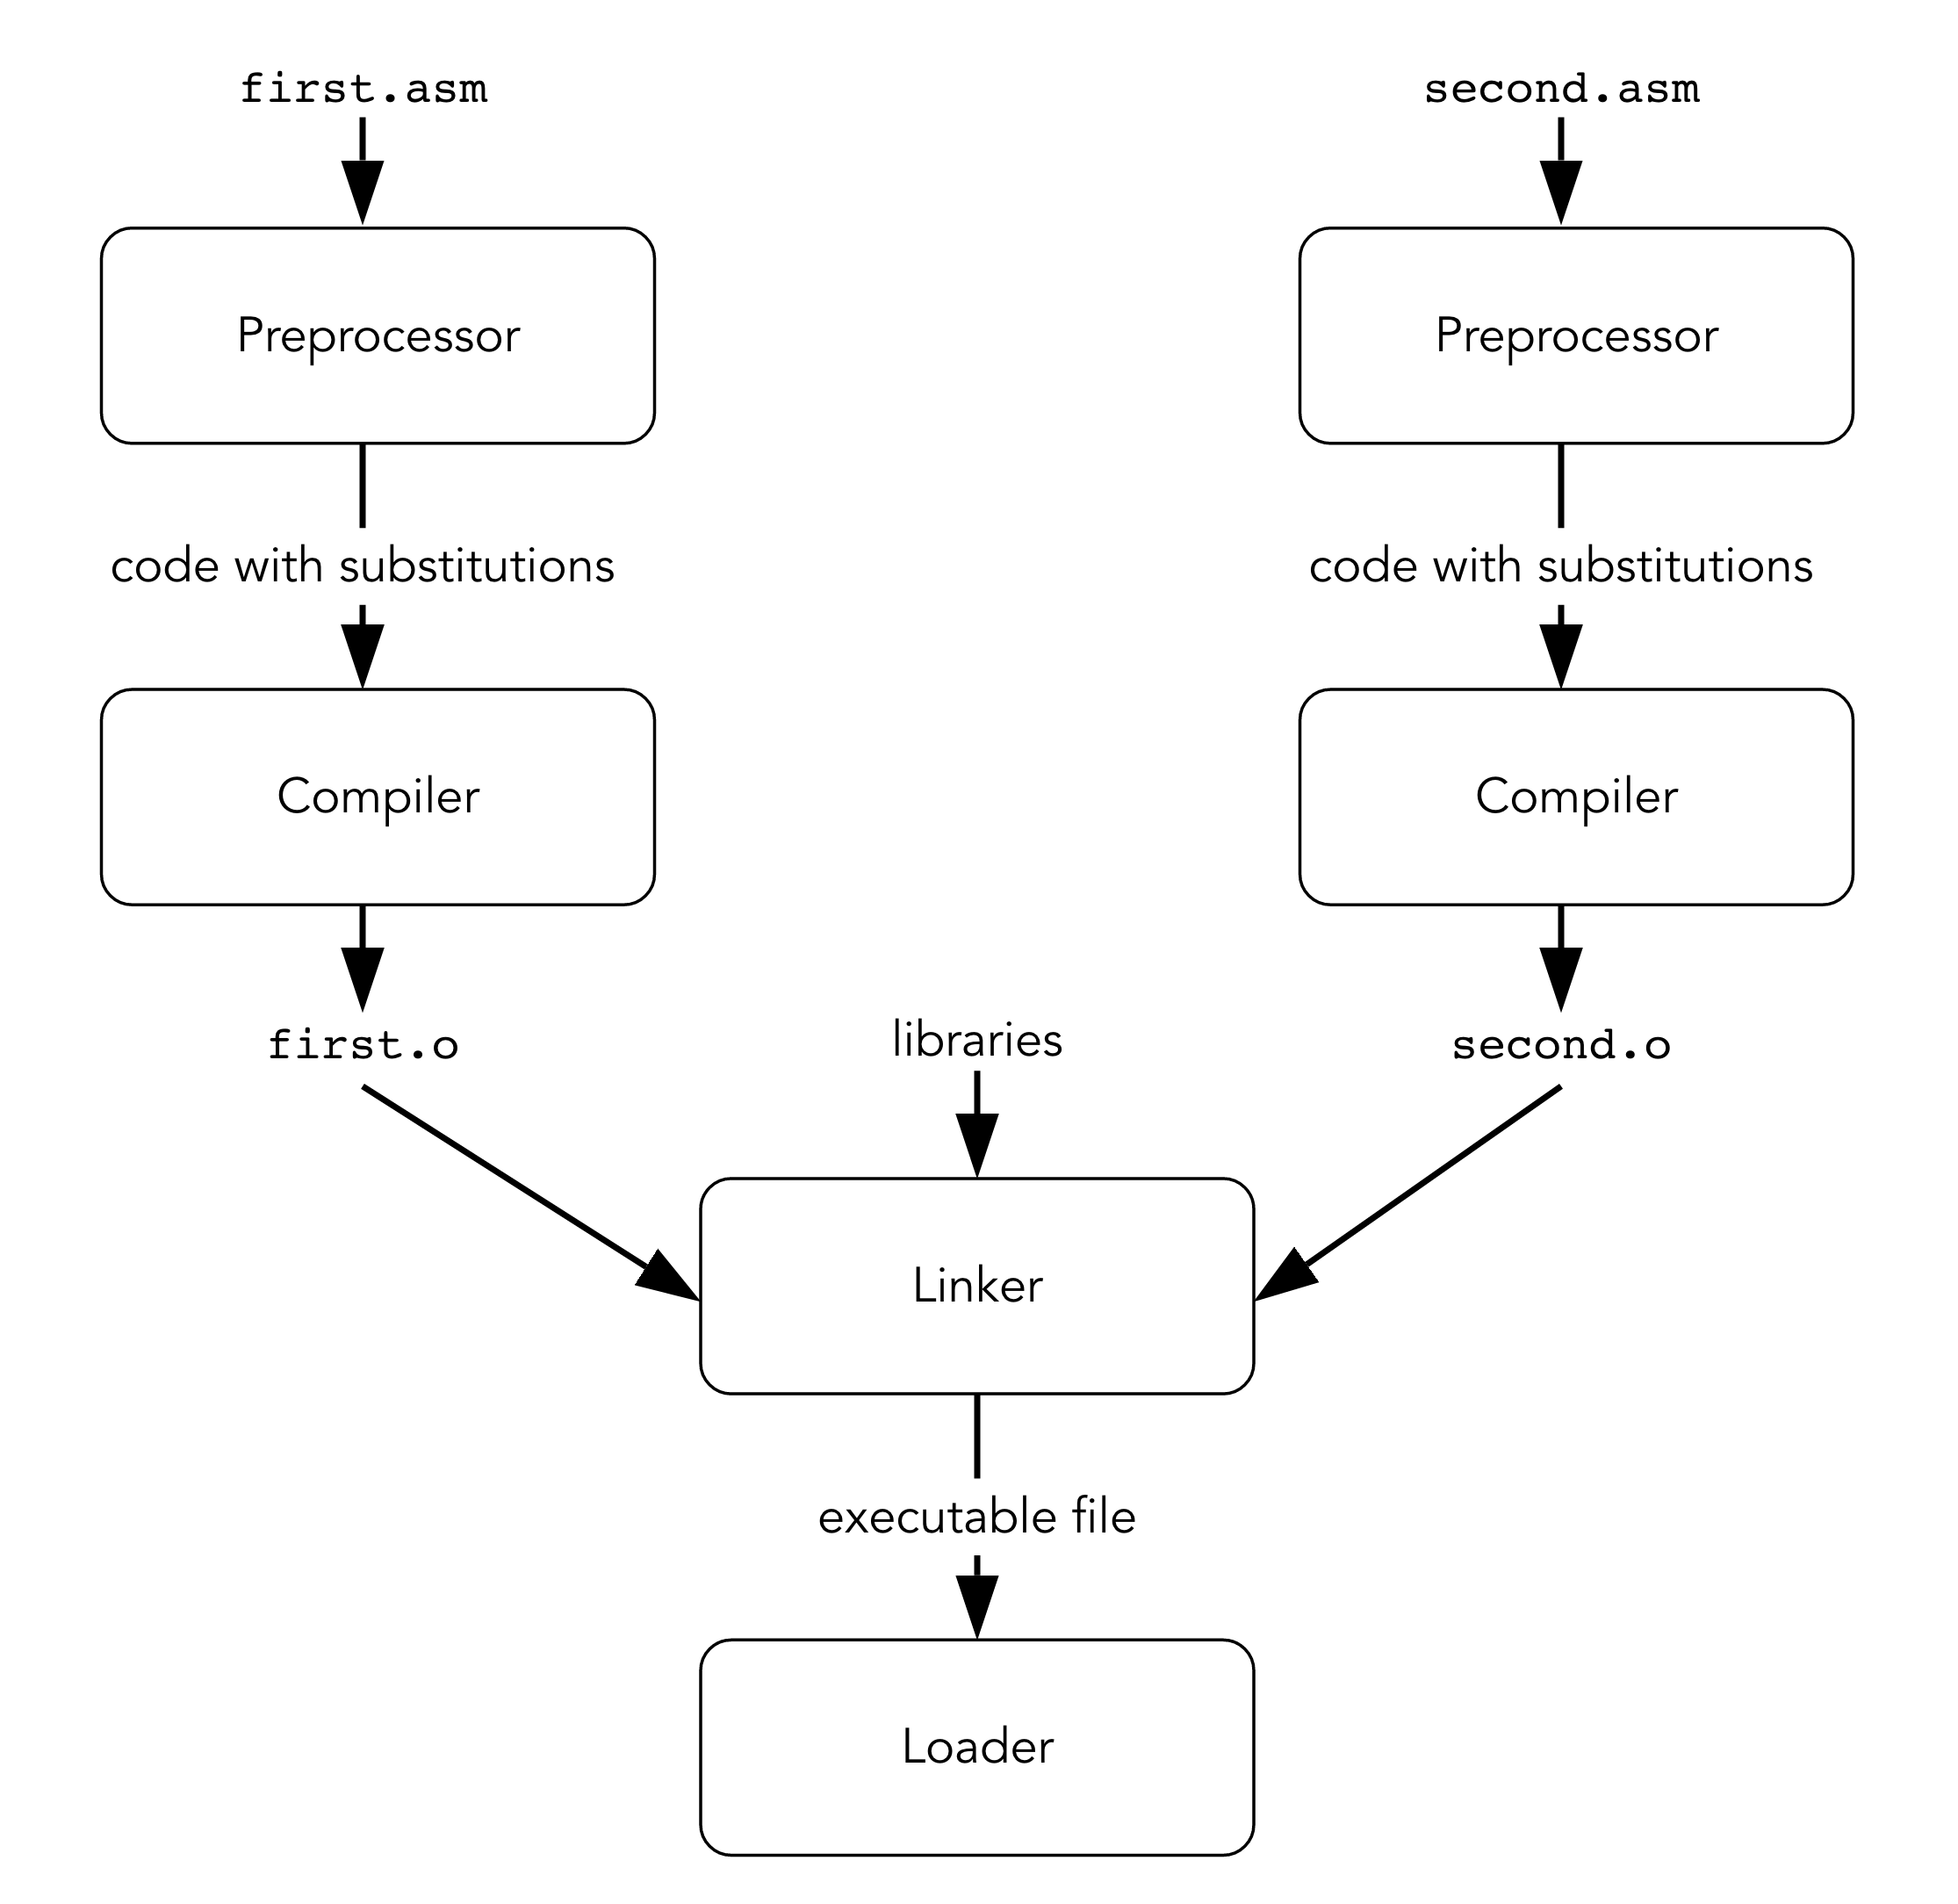
\includegraphics[height=\textheight]{images/compilation.png} 
\end{frame}


\begin{frame}{Compiling separately vs all at once}

\end{frame}

\begin{frame}{Particular interest}

\begin{itemize}
    \item  Separate compilation.
    \item  Using a separate program (linker) on the final stage.
\end{itemize}
\end{frame}

\begin{frame}{Why we need separate compilation?}
\begin{itemize}
    \item  Use code that is already compiled (libraries).
    \item  Don't recompile everything after each change (debug time explodes).

    \begin{itemize}
        \item  Some programs take \emph{hours} to compile.
    \end{itemize}
    
\end{itemize}
\end{frame}


\begin{frame}

\end{frame}
%\begin{frame}[allowframebreaks]
%\frametitle{References}
%\bibliography{biblio} 
%\end{frame}

\end{document}


